\documentclass[a4paper, 11pt]{article}
\usepackage{geometry}
\geometry{letterpaper, margin=1in}
\usepackage{graphicx}
\graphicspath{ {images/} }

\usepackage{amsmath}
\usepackage{amssymb}  
\usepackage{amsthm}
\usepackage{ulem} 


\usepackage{pdfpages} % for including full pdf pages

% format to allow bolded theorems, corollaries, etc... 
\newtheorem*{theorem}{Theorem}
\newtheorem*{corollary}{Corollary}
\newtheorem*{lemma}{Lemma}
\newtheorem*{definition}{Definition}
\newtheorem*{Example}{Example} 
\newtheorem*{Remark}{Remark}

% stop typing \mathbb a thousand times 
\newcommand{\R}{\mathbb{R}}
\newcommand{\C}{\mathbb{C}}
\newcommand{\F}{\mathbb{F}}

% commands for bra-ket notation
\newcommand{\bra}[1]{\ensuremath{\left\langle#1\right|}}
\newcommand{\ket}[1]{\ensuremath{\left|#1\right\rangle}}
\newcommand{\bracket}[2]{\ensuremath{\left\langle #1 \middle| #2 \right\rangle}}
\newcommand{\matrixel}[3]{\ensuremath{\left\langle #1 \middle| #2 \middle| #3 \right\rangle}}
\newcommand{\expectation}[1]{\ensuremath{\left\langle #1 \right\rangle}}

% change margins for solution
\newenvironment{solution}{%
	\begin{list}{}{%
			\setlength{\topsep}{0pt}%
			\setlength{\leftmargin}{1.5cm}%
			\setlength{\rightmargin}{1.5cm}%
			\setlength{\listparindent}{\parindent}%
			\setlength{\itemindent}{\parindent}%
			\setlength{\parsep}{\parskip}%
		}%
		\item[]}{\end{list}}



\begin{document}
%Header-Make sure you update this information!!!!
\noindent
\large\textbf{Homework 2} \hfill \textbf{John Waczak} \\
\normalsize PH 652 \hfill  Date: \today \\
Dr. Oksana Ostroverkhova  
\par\noindent\rule{\textwidth}{0.4pt} \\\\

\noindent 1. Consider a system which is initially in the state $\psi(\theta, \phi) = \frac{1}{\sqrt{5}}Y_1^{-1}(\theta,\phi)+\frac{\sqrt{3}}{\sqrt{5}}Y_1^0(\theta, \phi)+\frac{1}{\sqrt{5}}Y_1^1(\theta,\phi)$ \\

\noindent (a) Find $\expectation{L_+}$ \\ 
\begin{solution}
  \noindent First, recall the definition of the raising and lowering operators for angular momentum and their action on $\ket{\ell, m}$ states.
  \begin{align*}
    L_\pm &= L_x \pm iL_y \\
    L_\pm \ket{\ell, m} &= c_\pm \ket{\ell, m\pm1} \\
    c_\pm &= \hbar\sqrt{(\ell\mp m)(\ell \pm m + 1)} \\
    L_+\ket{\ell, \ell} &= 0 \\
    L_-\ket{\ell, -\ell} &= 0
  \end{align*}


  \noindent To make use of the ladder operators, we first observe that the state vector corresponding to $\psi$ is given by
  \begin{equation*}
    \ket{\psi} = \frac{1}{\sqrt{5}}\ket{1, -1} + \frac{\sqrt{3}}{\sqrt{5}}\ket{1,0} + \frac{1}{\sqrt{5}}\ket{1,1}
  \end{equation*}
  Now we can try to expand the expectation value
  \begin{align*}
    L_+\ket{\psi}&=L_+\Big(\frac{1}{\sqrt{5}}\ket{1, -1} + \frac{\sqrt{3}}{\sqrt{5}}\ket{1,0} + \frac{1}{\sqrt{5}}\ket{1,1}\Big) \\
    &= \frac{1}{\sqrt{5}}\hbar\sqrt{(1+1)(1-1+1)}\ket{1,0} + \frac{\sqrt{3}}{\sqrt{5}}\hbar\sqrt{1(1+1)}\ket{1,1} + 0 \\
    \Rightarrow \expectation{L_+} &= \Big(\frac{1}{\sqrt{5}}\bra{1, -1} + \frac{\sqrt{3}}{\sqrt{5}}\bra{1,0} + \frac{1}{\sqrt{5}}\bra{1,1}\Big)\Big(\frac{\sqrt{2}}{\sqrt{5}}\hbar\ket{1,0}+\frac{\sqrt{6}}{\sqrt{5}}\hbar\ket{1,1}\Big) \\
    &= \hbar\left( \frac{\sqrt{6}}{5} + \frac{\sqrt{6}}{5} \right) \\ 
    &= \frac{2\sqrt{6}}{5}\hbar
  \end{align*}

\noindent This is an interesting result although I am unsure how to interpret the final value as $L_+$ is not a Hermitian operator. \\
\end{solution}

\noindent (b) If $L_z$ were measured what values would one obtain and with what probabilities?\\
\begin{solution}
  \noindent Recall that $L_z\ket{\ell, m} = \hbar m \ket{\ell,m}$. Therefore, if we measured $L_z$ for incoming state $\ket{\psi}$, we would expect possible values $\{-\hbar, 0, \hbar\}$ with probabilities
  \begin{align*}
    P(m=-1) &= \bracket{m=-1}{\psi} = \left| \frac{1}{\sqrt{5}} \right|^2 = \frac{1}{5} \\
    P(m=0) &= \bracket{m=0}{\psi} = \left| \frac{\sqrt{3}}{\sqrt{5}} \right|^2 = \frac{3}{5} \\
    P(m=1) &= \bracket{m=1}{\psi} = \left| \frac{\sqrt{1}}{\sqrt{5}} \right|^2 = \frac{1}{5} \\
  \end{align*}

  \noindent \textbf{NOTE:} these probabilities sum to unity as expected.\\
\end{solution}


\noindent (c) If after measuring $L_z$ we find $l_z = -\hbar$, what are the uncertainties $\Delta L_x$ and $\Delta L_y$? \\
\begin{solution}
  \noindent Measuring $L_z$ with certainty to have $l_z=-\hbar$ means that the state $\ket{\psi}$ has been projected into $\ket{\psi}\rightarrow\ket{1,-1}$ (the only value of $\ell$ in $\ket{\psi}$ is 1). Now we recall the solution to the third problem from HW1 in which we showed that
  \begin{align*}
    \expectation{L_x} & = \expectation{L_y} = 0 \\
    \expectation{L_x^2} &= \expectation{L_y^2} = \frac{\ell(\ell+1)\hbar^2-m^2\hbar^2}{2}
  \end{align*}
  This indicates that the uncertainties $\Delta L_x$ and $\Delta L_y$ must be the same, i.e.
  \begin{equation*}
    \Delta L_x = \Delta L_y = \sqrt{\expectation{L_y}^2-\expectation{L_y}^2} = \sqrt{\frac{2\hbar^2-(-1)^2\hbar^2}{2}} = \frac{\hbar}{\sqrt{2}}
  \end{equation*}
\end{solution}

\noindent 2. Consider a system whose wave function is $\psi(x,y,z)=\frac{1}{4\sqrt{\pi}}\frac{2z^2-x^2-y^2}{r^2}+\sqrt{\frac{3}{\pi}}\frac{xz}{r^2}$\\

\noindent (a) Calculate $L^2\psi$ and $L_z\psi$. Find the total angular momentum of this particle.\\
\begin{solution}
  \noindent To begin, we would like to change the coordinates to $\{r, \theta, \phi \}$ in order to be able to apply the various angular momentum operators. Recall that Cartesian coordinates are related to spherical coordinates by
  \begin{align*}
    x &= r\sin\theta\cos\phi \\
    y &= r\sin\theta\sin\phi \\
    z &= r\cos\theta
  \end{align*}
  applying these transformations yields
  \begin{align*}
    \psi(r,\theta,\phi) &= \frac{1}{4\sqrt{\pi}}\frac{2r^2\cos^2\theta-r^2\sin^2\theta\cos^2\phi-r^2\sin^2\theta\sin^2\phi}{r^2}+\sqrt{\frac{3}{\pi}}\frac{r^2\sin\theta\cos\phi\cos\theta}{r^2} \\
    &= \frac{1}{4\sqrt{\pi}}\left( 2\cos^2\theta-\sin^2\theta\cos^2\phi-\sin^2\theta\sin^2\phi  \right) + \sqrt{\frac{3}{\pi}}\sin\theta\cos\theta\cos\phi
  \end{align*}
  Thus, we can see that in fact, $\psi=\psi(\theta,\phi)$. In other words, $\psi$ is strictly a function of angle and therefore may be decomposed into the complete orthonormal basis of spherical harmonics $Y_\ell^m(\theta,\phi)$ where the expansion coefficients are given by
  \begin{equation*}
    c_{\ell, m} = \bracket{\ell,m}{\psi}= \int_0^\pi \int_0^{2\pi} \Big(Y_\ell^m(\theta,\phi)\Big)^*\psi(\theta,\phi)\sin\theta d\phi d\theta
  \end{equation*}
  \textbf{Note:} we must make sure to include the solid angle element $d\Omega = \sin\theta d\theta d\phi$ when changing coordinates. I performed the integrals for $\ell\in\{0, 1, 2\}$ and $m\in\{-\ell, ..., \ell\}$ using Mathematica (to save time). They are shown on the following page.

  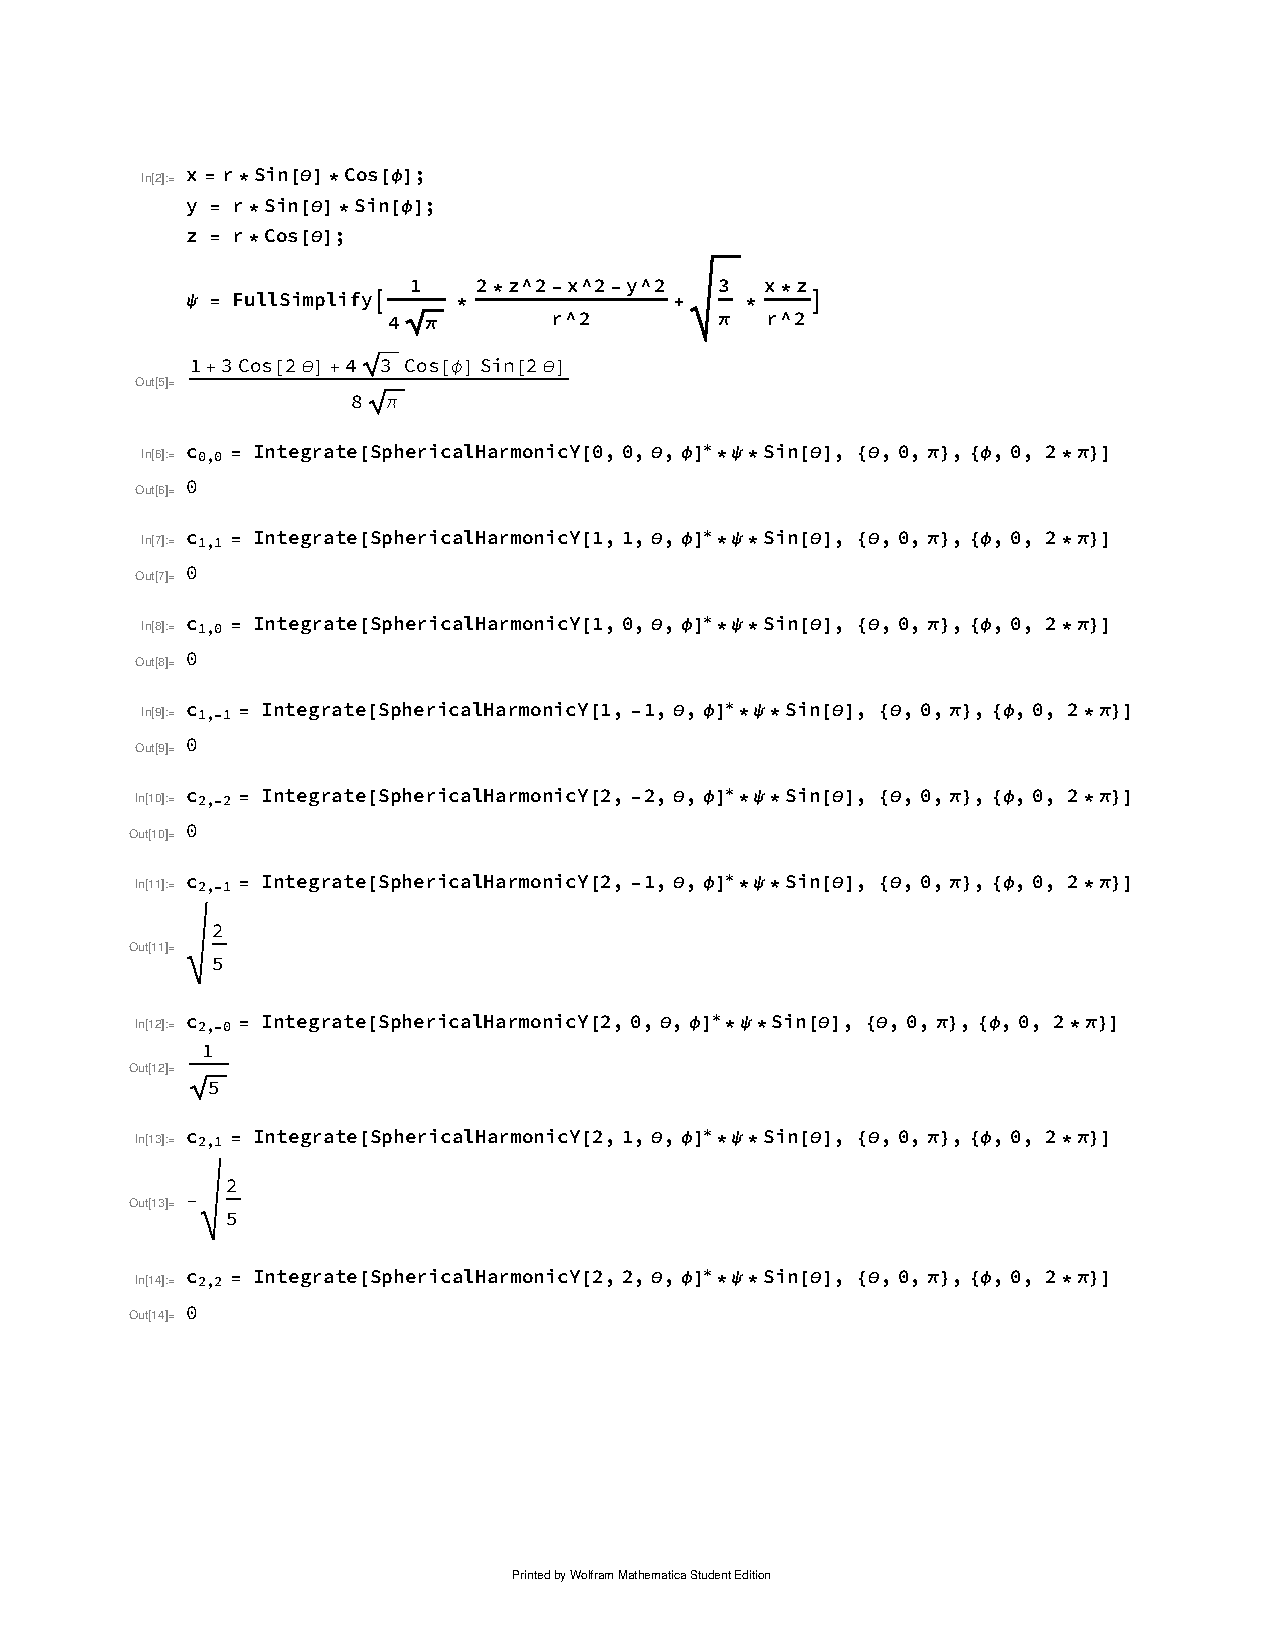
\includepdf{Problem2}

  \noindent From these integrals, we can see that we have found all of the necessary coefficients as the sum of their squared norms is unity. Now we can rewrite the wavefunction as
  \begin{align*}
    \psi(\theta,\phi) &= \sqrt{\frac{2}{5}}Y_2^{-1}(\theta,\phi)+\sqrt{\frac{1}{5}}Y_2^0(\theta, \phi)-\sqrt{\frac{2}{5}}Y_2^1(\theta,\phi) \\
    \Rightarrow \ket{\psi} &= \sqrt{\frac{2}{5}}\ket{2,-1} + \sqrt{\frac{1}{5}}\ket{2,0}-\sqrt{\frac{2}{5}}\ket{2,1}
  \end{align*}
  From this representation we can easily compute $L^2$ acting on this state as the operator is linear and we have only one value of $\ell$.
  \begin{align*}
    L^2\ket{\psi}&= 2(2+1)\hbar^2\left( \sqrt{\frac{2}{5}}\ket{2,-1}+\sqrt{\frac{1}{5}}\ket{2,0}-\sqrt{\frac{2}{5}}\ket{2,1}\right) \\
    &= 6\hbar^2 \left( \sqrt{\frac{2}{5}}\ket{2,-1}+\sqrt{\frac{1}{5}}\ket{2,0}-\sqrt{\frac{2}{5}}\ket{2,1}\right) \\
    &= 6\hbar \ket{\psi} 
  \end{align*}
  Interestingly, this turned out to be a regular eigenvalue equation. The calculation for $L_z$ is as follows
  \begin{align*}
    L_z\ket{\psi} &= -\sqrt{\frac{2}{5}}\hbar\ket{2,-1} + 0\ket{2,0} -\sqrt{\frac{2}{5}}\hbar\ket{2,1} \\
  \end{align*}

  \noindent So for $L_z$ we do not have an eigenvalue equation. Because $L^2\ket{\psi}$ is an eigenvalue equation, we can define the total angular momentum to be given by the square root of the eigenvalue, i.e.
  \begin{equation*}
    |\vec{L}| = \hbar\sqrt{6}
  \end{equation*}
\end{solution}

\noindent (b) Calculate $L_+\ket{\psi}$ and $\matrixel{\psi}{L_+}{\psi}$\\
\begin{solution}
  \noindent We have that
  \begin{align*}
    L_+\ket{\psi} &= L_+\left( \sqrt{\frac{2}{5}}\ket{2,-1} + \sqrt{\frac{1}{5}}\ket{2,0}-\sqrt{\frac{2}{5}}\ket{2,1}\right) \\
    &= \hbar\sqrt{(2-(-1))(2+(-1)+1)}\sqrt{\frac{2}{5}}\ket{2,0}\\
    &\hspace{5em}+\hbar\sqrt{(2-0)(2+0+1)}\sqrt{\frac{1}{5}}\ket{2,1}\\
    &\hspace{5em}-\hbar\sqrt{(2-1)(2+1+1)}\ket{2,2} \\
    &= \hbar\sqrt{6}\sqrt{\frac{2}{5}}\ket{2,0}+\hbar\sqrt{6}\sqrt{\frac{1}{5}}\ket{2,1}-\hbar\sqrt{4}\sqrt{\frac{2}{5}}\ket{2,2} \\
    &= \hbar\sqrt{\frac{12}{5}}\ket{2,0}+\hbar\sqrt{\frac{6}{5}}\ket{2,1}-\hbar 2\sqrt{\frac{2}{5}}\ket{2,2} 
  \end{align*}
  I thought to renormalize this however this quantity now has dimensions of angular momentum so renormalizing doesn't really make sense. \\

  \begin{align*}
    \matrixel{\psi}{L_+}{\psi} &= \left(\sqrt{\frac{2}{5}}\bra{2,-1}+\sqrt{\frac{1}{5}}\bra{2,0}-\sqrt{\frac{2}{5}}\bra{2,1} \right)\left(  \hbar\sqrt{\frac{12}{5}}\ket{2,0}+\hbar\sqrt{\frac{6}{5}}\ket{2,1}-\hbar 2\sqrt{\frac{2}{5}}\ket{2,2} \right)\\
    &= \hbar\frac{\sqrt{12}}{5}-\hbar\frac{\sqrt{12} }{5} = 0 
  \end{align*}
  Once again, we find an interesting result for the expectation value but I am at a loss on how to interpret this as there is no physical measurement corresponding to $L_+$. \\ 
\end{solution}


\noindent (c) If a measurement of $L_z$ is carried out, what values would one obtain and with what probabilities?\\

\begin{solution}
  \noindent We have the state
  \begin{equation*}
    \ket{\psi} = \sqrt{\frac{2}{5}}\ket{2,-1} + \sqrt{\frac{1}{5}}\ket{2,0}-\sqrt{\frac{2}{5}}\ket{2,1} 
  \end{equation*}
  where, as in problem 1, the eigenvalue equation $L_z\ket{\ell,m}= \hbar m \ket{\ell,m}$ holds. Therefore the possible values are $\{-\hbar, 0, \hbar\}$ and they occur with probability
  \begin{align*}
    P(m=-1) &= \bracket{m=-1}{\psi} = \left| \sqrt{\frac{2}{5}}\right|^2 = \frac{2}{5}\\
    P(m=0) &= \bracket{m=0}{\psi} = \left| \sqrt{\frac{1}{5}}\right|^2 = \frac{1}{5}\\
    P(m=1) &= \bracket{m=1}{\psi} = \left| -\sqrt{\frac{2}{5}}\right|^2 = \frac{2}{5}
  \end{align*}

\end{solution}

\noindent 3. Read ``Fullerene Quantum Gyroscope'' and answer the following...\\

\noindent 1) What is the claim of the paper?\\
\begin{solution}\noindent\textbf{The authors claim to have observed quantized rotational states of $C_2$ units in fullerene\\}\end{solution}

\noindent 2) Did the authors do experiment, calculations, or both?\\
\begin{solution}\noindent\textbf{The authors performed both experiment (Raman spectroscopy) and calculations (DFT) }\\\end{solution}

\noindent 3) What kind of experiment did the authors do? \\ 
\begin{solution}\noindent\textbf{The authors performed Raman spectroscopy.\\}\end{solution}
\noindent4) What are the measured quantities?\\
\begin{solution}\noindent\textbf{Line positions and widths were measured with 1.5 $cm^{-1}$ resolution in response to both red and green laser excitation. Particularly, the line positions (and their spacing) are suggestive of planar rotational modes.\\}\end{solution}

\noindent 5) How is the experimentally measured line separation (see Fig.2) related to the difference in energy levels (e.g. $E_\ell-E_{\ell-1}$)?  \\
\begin{solution}\noindent\textbf{As explained on the second page of the article, the authors use the reciprocal length units for the rotational constant (that is why the Raman shift is measured in cm-1 rather than in energy units). The conversion is
    \begin{equation*}
      \overline{B} = \frac{B}{hc} = \frac{h}{8\pi^2cI} = \frac{\hbar}{4\pi c\mu r_e^2} 
    \end{equation*}
    which assumes $h,c$ are in cgs units. NOTE: I figured this out by searching through wikipedia. Furthermore, by the Einstein-Plank relation, we have that
    \begin{equation*}
      E = h\nu = \hbar c k
    \end{equation*}
    putting these together yields
    \begin{equation*}
      k = \frac{B}{\hbar c}\ell(\ell+1)
    \end{equation*}
    Experiment measures light corresponding to the transition between energy levels and therefore we want to look at $E_{\ell, \ell-1}$ as well as the distance between these transitions $k_{\ell+1,\ell}-k_{\ell,\ell-1}$ as is detailed in question 7.\\}\end{solution}


\noindent6) In the first column of page 2, the authors state that if the motion of the rotator is confined to a plane, then the energies are $E(m)=Bm^2$. Why?  \\
\begin{solution}\noindent\textbf{If the motion is confined to the plane, $\theta\rightarrow  \text{constant}$ we no longer have a rigid rotor but rather a particle confined to a ring whose energy spectrum is $E_m = Bm^2$ because in this special case $L^2=L_z^2$.\\}\end{solution}

\noindent 7) What are the selection rules for Raman scattering? What line separation is expected and why?  \\
\begin{solution}\noindent\textbf{The selection rules are
    \begin{align*}
      \Delta \ell &= \pm 2 \qquad \Delta m = \pm2
    \end{align*}
    This means that for both cases, the expected line separation is 8B. We can see this by examining the energy of these transitions. 
    \begin{align*}
      k = \frac{E}{\hbar c}\\
      E_{\ell, \ell-2} &= B(\ell(\ell+1)-(\ell-2)(\ell-1)) \\
      &= B(4\ell-2) \\
      E_{\ell+2, \ell} &= B((\ell+2)(\ell+3)-\ell(\ell+1)) \\
      &= B(4\ell+6) \\
      \Rightarrow k_{\ell+2,\ell}-k_{\ell,\ell-2} &= \frac{B}{\hbar c}(4\ell+6-4\ell+2)= 8\frac{B}{\hbar c}
    \end{align*}
    This is the same for the plane rotor case
    \begin{align*}
      E(m) &= Bm^2 \\
      E_{m,m-2} &= B(m^2-(m-2)^2) \\
      &= B(m^2-m^2+4m-4) = B(4m-4)  \\
      E_{m+2, m} &= B((m+2)^2-m^2) \\
      & = B(m^2+4m+4-m^2)=B(4m+4) \\ 
      k_{m+2,m}-k_{m,m-2} &= \frac{B}{\hbar c}(4m+4-4m+4)= 8\frac{B}{\hbar c}
    \end{align*} }\end{solution}
\noindent 8) How is the rotational constant B derived from the experimental data? What is the obtained value for B? \\
\begin{solution}\noindent\textbf{Using the results from the previous question we have an equation relating the line spacing directly to B. Inverting the equation gives
    \begin{equation*}
      B = \hbar c \Delta k/8
      \end{equation*}\\}\end{solution}

\noindent 9) What are the obtained values for the moment of intertia and the distance between the atoms (i.e. $r_e$)? \\
\begin{solution}\noindent\textbf{The moment of inertia was found to be $1.617\times10^{-46}$ $kgm^2$. This gives a C-C length of $0.127$ $nm$.  \\}\end{solution}

\noindent10) Under what conditions is the model of an unperturbed rotator applicable to this ``real'' system?\\
\begin{solution}\noindent\textbf{The experimental results follow closely for the unperturbed plane rotor for higher transitions. In the low energy range, more lines were observed than expected.\\}\end{solution}

\noindent 11) What do the authors introduce in the Schrodinger equation to better describe the experimental results? \\
\begin{solution}\noindent\textbf{The authors introduces a ``rotational potential barrier''  which they model with a cosine function
    \begin{equation*}
      V(\gamma) = V_0(1-\cos4\gamma)/2
    \end{equation*}
    I assume that the paper uses $\gamma$ as the planar angle which we have called $\phi$ as they describe the perturbation as being for the plan rotor. \\}\end{solution}

\noindent 12) Which model provides a better agreement with the experiment (see Table I)? \\
\begin{solution}\noindent\textbf{Based off of Table 1 it appears that the perturbed plane rotor gives the best agreement with experiment as it matches the unperturbed plane rotor values for the highest three transitions but is also the closest for the lower transitions.\\}\end{solution}
























\end{document}



























